
\begin{center}
{
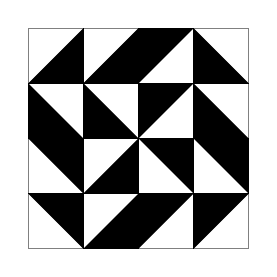
\begin{tikzpicture}[scale=0.7]
 \draw [step=1cm,gray,very thin](0,-1) grid (4,3); 
 \draw[opacity=1,fill=black](0,0)--(1,0)--(1,-1); 
 \draw[opacity=1,fill=black](0,1)--(1,1)--(1,0); 
 \draw[opacity=1,fill=black](1,1)--(0,1)--(0,2); 
 \draw[opacity=1,fill=black](1,3)--(1,2)--(0,2); 
 \draw[opacity=1,fill=black](2,0)--(2,-1)--(1,-1); 
 \draw[opacity=1,fill=black](2,1)--(2,0)--(1,0); 
 \draw[opacity=1,fill=black](2,1)--(1,1)--(1,2); 
 \draw[opacity=1,fill=black](2,3)--(2,2)--(1,2); 
 \draw[opacity=1,fill=black](2,-1)--(2,0)--(3,0); 
 \draw[opacity=1,fill=black](2,1)--(3,1)--(3,0); 
 \draw[opacity=1,fill=black](2,1)--(2,2)--(3,2); 
 \draw[opacity=1,fill=black](2,2)--(2,3)--(3,3); 
 \draw[opacity=1,fill=black](3,-1)--(3,0)--(4,0); 
 \draw[opacity=1,fill=black](3,1)--(4,1)--(4,0); 
 \draw[opacity=1,fill=black](4,1)--(3,1)--(3,2); 
 \draw[opacity=1,fill=black](4,2)--(3,2)--(3,3); 
\end{tikzpicture}

\textit{The 0011 pattern}
}
\end{center}
